Ci-dessous les différentes situations avec les screenshots avec description montrant la réalisation de ses points :

\begin{itemize}
    \item \textcolor{green}{[A1] Constitution d’un groupe :}
    %inserer screenshot et description
    \\Comme vu dans section1, nous avons constituer un groupe de 2 personne avec Achraf et Jolan.
    \begin{figure}[h]
    \centering
    \fbox{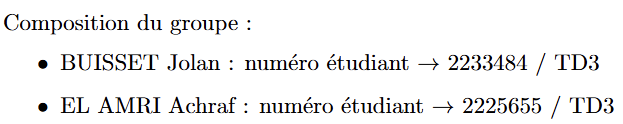
\includegraphics[width=0.5\textwidth]{screenshots/compositionGRP.png}}
    \end{figure}
    \\ce qui fait que nous validons la mise en situation A1.

    \item \textcolor{green}{[A2] Dépôt git en ligne : }
    %inserer screenshot et description
    \\Pour valider A2, nous vous donnons ici le lien URL de notre dépot github : 
    \url{https://github.com/JolanB110/projet-git/tree/main}

    Vous avez désormais accès a notre dépot en ligne, nous avons donc validé la mise en situation A2.
    
    \item \textcolor{green}{[A3] Intégration des contributions : }
    %inserer screenshot et description
    \\ Pour la réalisation du projet, nous avons tout les 2 effectuer des commits afin de la plus équitable des manières afin de correspondre a la mise en situation :\\

    \begin{figure}[h]
    \centering
    \fbox{\includegraphics[width=0.5\textwidth]{screenshots/intégration-achraf.png}}
    \end{figure}
    \begin{figure}[h]
    \centering
    \fbox{\includegraphics[width=0.5\textwidth]{screenshots/intégration-jolan.png}}
    \end{figure}
    Nous avons donc validée la mise en situation A3.

    \item \textcolor{orange}{[B1] Gestion par branches : }
    \\ Voici l'ensemble des branches : \\ 
    \fbox{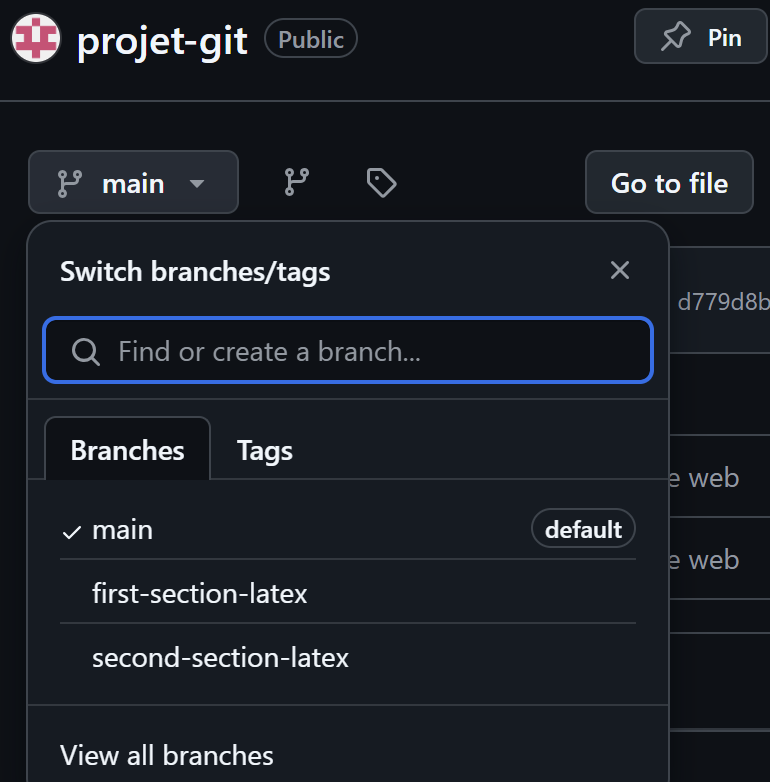
\includegraphics[width=0.5\textwidth]{screenshots/brancheLatex.png}}
    \item \textcolor{orange}{[B2] Intégration de version et tag : }
    %inserer screenshot et description
    \item \textcolor{orange}{[B3] Gestion des propositions de contributions : }
    %inserer screenshot et description
    \item \textcolor{orange}{[B4] Intégration de site web : }
    %inserer screenshot et description
    \item \textcolor{red}{[C1] Répartition de taches et milestone : }
    %inserer screenshot et description
    \item \textcolor{red}{[C2] Intégration continue : }
    %inserer screenshot et description
    \item \textcolor{red}{[C3] Gestion de submodule : }
    %inserer screenshot et description
\end{itemize}